% !TeX program = XeLaTeX
\documentclass[UTF8,a4paper,12pt,fontset=none]{ctexrep}
\usepackage[a4paper,margin=2.5cm]{geometry}
\usepackage{graphicx}
\usepackage{float}
\usepackage{array}
\usepackage{longtable}
\usepackage{booktabs}
\usepackage{caption}
\usepackage{enumitem}
\usepackage{hyperref}
\usepackage{titlesec}
\usepackage{setspace}
\usepackage{xcolor}
\usepackage{fancyhdr}
\usepackage{lastpage}
\usepackage{etoolbox}

\hypersetup{
  colorlinks=true,
  linkcolor=black,
  urlcolor=black,
  citecolor=black,
  pdftitle={校园学术活动智能推荐平台项目开发计划书}
}

\setmainfont{TeX Gyre Termes}
\setsansfont{TeX Gyre Heros}
\setmonofont{Latin Modern Mono}
\setCJKmainfont{Noto Serif CJK SC}
\setCJKsansfont{Noto Sans CJK SC}
\setCJKmonofont{Noto Sans Mono CJK SC}
\newcommand{\songti}{\rmfamily}
\newcommand{\heiti}{\sffamily}

\definecolor{ZJUBlue}{RGB}{0, 63, 136}
\setcounter{secnumdepth}{3}
\setcounter{tocdepth}{3}
\setlength{\parindent}{2em}
\setlength{\parskip}{0.35em}
\setlength{\headheight}{15pt}
\setlength{\LTpre}{0.85\baselineskip}
\setlength{\LTpost}{0.75\baselineskip}
\setlength{\intextsep}{0.8\baselineskip}
\setlength{\textfloatsep}{0.9\baselineskip}
\setlength{\tabcolsep}{4pt}
\renewcommand{\arraystretch}{1.3}
\onehalfspacing
\captionsetup{font=small,labelfont=bf,labelsep=quad}
\captionsetup[figure]{justification=centering}

\ctexset{
  chapter = {
    name = {第,章},
    number = \arabic{chapter},
    format = \centering\heiti\zihao{3},
    beforeskip = 18pt,
    afterskip = 24pt
  },
  section = {
    format = \bfseries\zihao{4}\color{ZJUBlue},
    beforeskip = 10pt,
    afterskip = 8pt
  },
  subsection = {
    format = \bfseries\zihao{-4},
    beforeskip = 8pt,
    afterskip = 6pt
  },
  subsubsection = {
    format = \bfseries\zihao{5},
    beforeskip = 6pt,
    afterskip = 4pt
  }
}

\pagestyle{fancy}
\fancyhf{}
\fancyhead[L]{项目开发计划书}
\fancyhead[R]{\nouppercase{\leftmark}}
\fancyfoot[C]{第 \thepage 页\ /\ 共 \pageref*{LastPage} 页}
\renewcommand{\headrulewidth}{0.6pt}
\renewcommand{\footrulewidth}{0.4pt}
\fancypagestyle{plain}{
  \fancyhf{}
  \fancyhead[L]{项目开发计划书}
  \fancyhead[R]{\nouppercase{\leftmark}}
  \fancyfoot[C]{第 \thepage 页\ /\ 共 \pageref*{LastPage} 页}
  \renewcommand{\headrulewidth}{0.6pt}
  \renewcommand{\footrulewidth}{0.4pt}
}

\newcommand{\reportuniversity}{浙江大学}
\newcommand{\reportcourse}{软件工程}
\newcommand{\reportdoctype}{课程设计报告}
\newcommand{\reportcovername}{项目开发计划书}
\newcommand{\reporttitlemain}{校园学术活动智能推荐平台}
\newcommand{\reporttitlesub}{项目开发计划书}
\newcommand{\reportadvisor}{邓水光}
\newcommand{\reportteamlineone}{黄晗\quad 宫上珺\quad 孟祥烨}
\newcommand{\reportteamlinetwo}{李妍雅\quad 庞星磊\quad 朱致远}
\newcommand{\reportdate}{\number\year\quad 年\quad \number\month\quad 月\quad \number\day\quad 日}
\newcommand{\coverfill}[2]{\underline{\makebox[#1][l]{#2}}}

\newcommand{\makecoursecover}{
  \begin{titlepage}
    \thispagestyle{empty}
    \centering
    \vspace*{1.0cm}
    
\includegraphics[width=0.42\textwidth]{figures/zju_title.png}\par
    \vspace{1.4cm}
    {\songti\zihao{2} \reportcovername \par}
    \vspace{1.6cm}
    
\includegraphics[width=0.30\textwidth]{figures/zju_logo.png}\par
    \vspace{1.5cm}
    \begin{minipage}{0.78\textwidth}
      \raggedright
      \renewcommand{\arraystretch}{1.85}
      {\songti\zihao{-3}
      \begin{tabular}{@{}p{2.5cm}p{9.4cm}@{}}
        项目主题： & \coverfill{8.6cm}{校园学术活动智能推荐平台} \\
        任课老师： & \coverfill{4.8cm}{\reportadvisor} \\
        项目组员： &
        \begin{tabular}[t]{@{}l@{}}
          \coverfill{8.6cm}{\reportteamlineone} \\
          \coverfill{8.6cm}{\reportteamlinetwo}
        \end{tabular} \\
      \end{tabular}\par}
    \end{minipage}
    \vfill
    {\songti\zihao{4} \reportdate \par}
  \end{titlepage}
}

\newcommand{\reporttable}[1]{\small #1}

\begin{document}
\pagenumbering{gobble}
\makecoursecover
\clearpage
\pagenumbering{Roman}
\tableofcontents
\clearpage
\pagenumbering{arabic}
\setcounter{page}{1}

\chapter{项目概述}

\section{项目背景简述}
校园学术活动信息通常分散在学院官网、通知页面、公众号和群消息中，存在检索困难、更新不同步、时间冲突难判断等问题。校园学术活动智能推荐平台希望将活动聚合、筛选推荐、课表导入、冲突检测、加入日程和日历展示整合到一个统一入口，帮助师生更高效地安排学术活动。

\chapter{开发范围}

\section{第一阶段开发范围}
\begin{longtable}{|p{0.16\textwidth}|p{0.34\textwidth}|p{0.38\textwidth}|}
\hline
\textbf{模块} & \textbf{第一阶段开发内容} & \textbf{预期效果} \\
\hline
用户认证 & 简化登录、注册、Token 鉴权 & 用户可进入系统 \\
\hline
活动浏览 & 活动列表、分页、详情页 & 用户可浏览活动信息 \\
\hline
搜索筛选 & 关键词、类别、学院、校区、时间筛选 & 用户可快速定位活动 \\
\hline
推荐模块 & 基于标签、热度、时间的规则推荐 & 首页展示推荐活动 \\
\hline
课表导入 & 手动录入、CSV/Excel 导入，OCR 作为加分项 & 用户课程可进入日历 \\
\hline
冲突检测 & 活动与课程/已有日程时间重叠判断 & 加入活动前提示冲突 \\
\hline
日历展示 & 展示课程、活动、冲突、推荐状态 & 用户可查看个人安排 \\
\hline
ICS 导出 & 导出活动或个人日程 & 可导入第三方日历 \\
\hline
后台管理 & 活动新增、编辑、下架、爬虫数据修正 & 管理员可维护活动 \\
\hline
爬虫数据 & 先采集一个学院的活动数据 & 提供真实活动样例 \\
\hline
\end{longtable}

\section{暂缓开发功能}
\begin{longtable}{|p{0.36\textwidth}|p{0.50\textwidth}|}
\hline
\textbf{暂缓功能} & \textbf{原因} \\
\hline
统一身份认证 SSO/CAS & 接入复杂，第一阶段使用本地账号替代 \\
\hline
精确地图通勤测算 & 依赖外部 API，先预留字段 \\
\hline
学术组队 & 与主流程关系较弱，后续扩展 \\
\hline
笔记共享与评价 & 属于社交沉淀功能，第二阶段再做 \\
\hline
个人学术轨迹 & 依赖大量历史数据，第一阶段不优先 \\
\hline
复杂 NLP 自动打标 & 先用人工标签或简单关键词规则 \\
\hline
协同过滤推荐 & 第一阶段使用规则推荐即可 \\
\hline
\end{longtable}

\section{最小可交付版本说明}
最小可交付版本至少应支持用户登录、活动列表展示、活动详情查看、关键词搜索、课表导入、加入日程、冲突检测、日历展示和 ICS 导出。即使爬虫、OCR 或推荐算法未完全完善，也必须通过样例数据和规则推荐保证完整演示流程可运行。

\chapter{总体开发方案}
目前我们其实已经初步搭建了项目框架，如下图所示：

    \begin{center}
    \begin{tabular}{cc}
      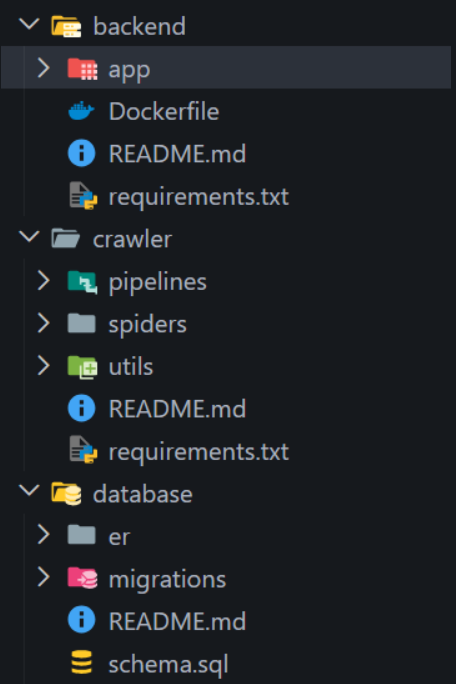
\includegraphics[width=0.46\textwidth]{figures/image-3.png} &
      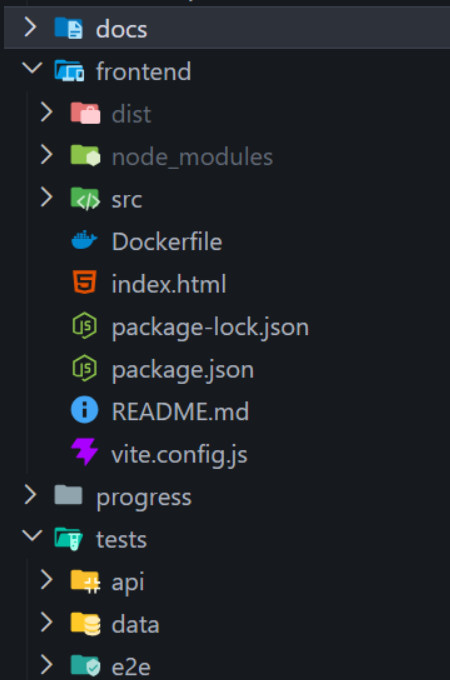
\includegraphics[width=0.46\textwidth]{figures/image-4.png}
    \end{tabular}
    \end{center}

\begin{verbatim}
SE-project/
├── frontend/                 # 前端项目，负责页面和交互
├── backend/                  # 后端项目，负责 API 和业务逻辑
├── crawler/                  # 爬虫脚本，负责采集学院活动数据
├── database/                 # 数据库建表、种子数据、ER 图
├── docs/                     # 项目文档、需求文档、接口规范、测试文档
├── tests/                    # 自动化测试、接口测试、测试数据
├── progress/                 # 成员个人开发日志和项目进度记录
├── README.md                 # 项目总说明
└── docker-compose.yml        # 后期可选，一键启动服务
\end{verbatim}

\section{系统总体架构}
系统采用前后端分离架构：前端负责页面展示和交互，后端负责业务逻辑、接口服务、权限控制、冲突检测和 ICS 文件生成，数据库负责存储用户、活动、课表、日程和标签数据，爬虫模块负责从学院站点采集活动信息并写入数据库。

\begin{figure}[H]
\centering
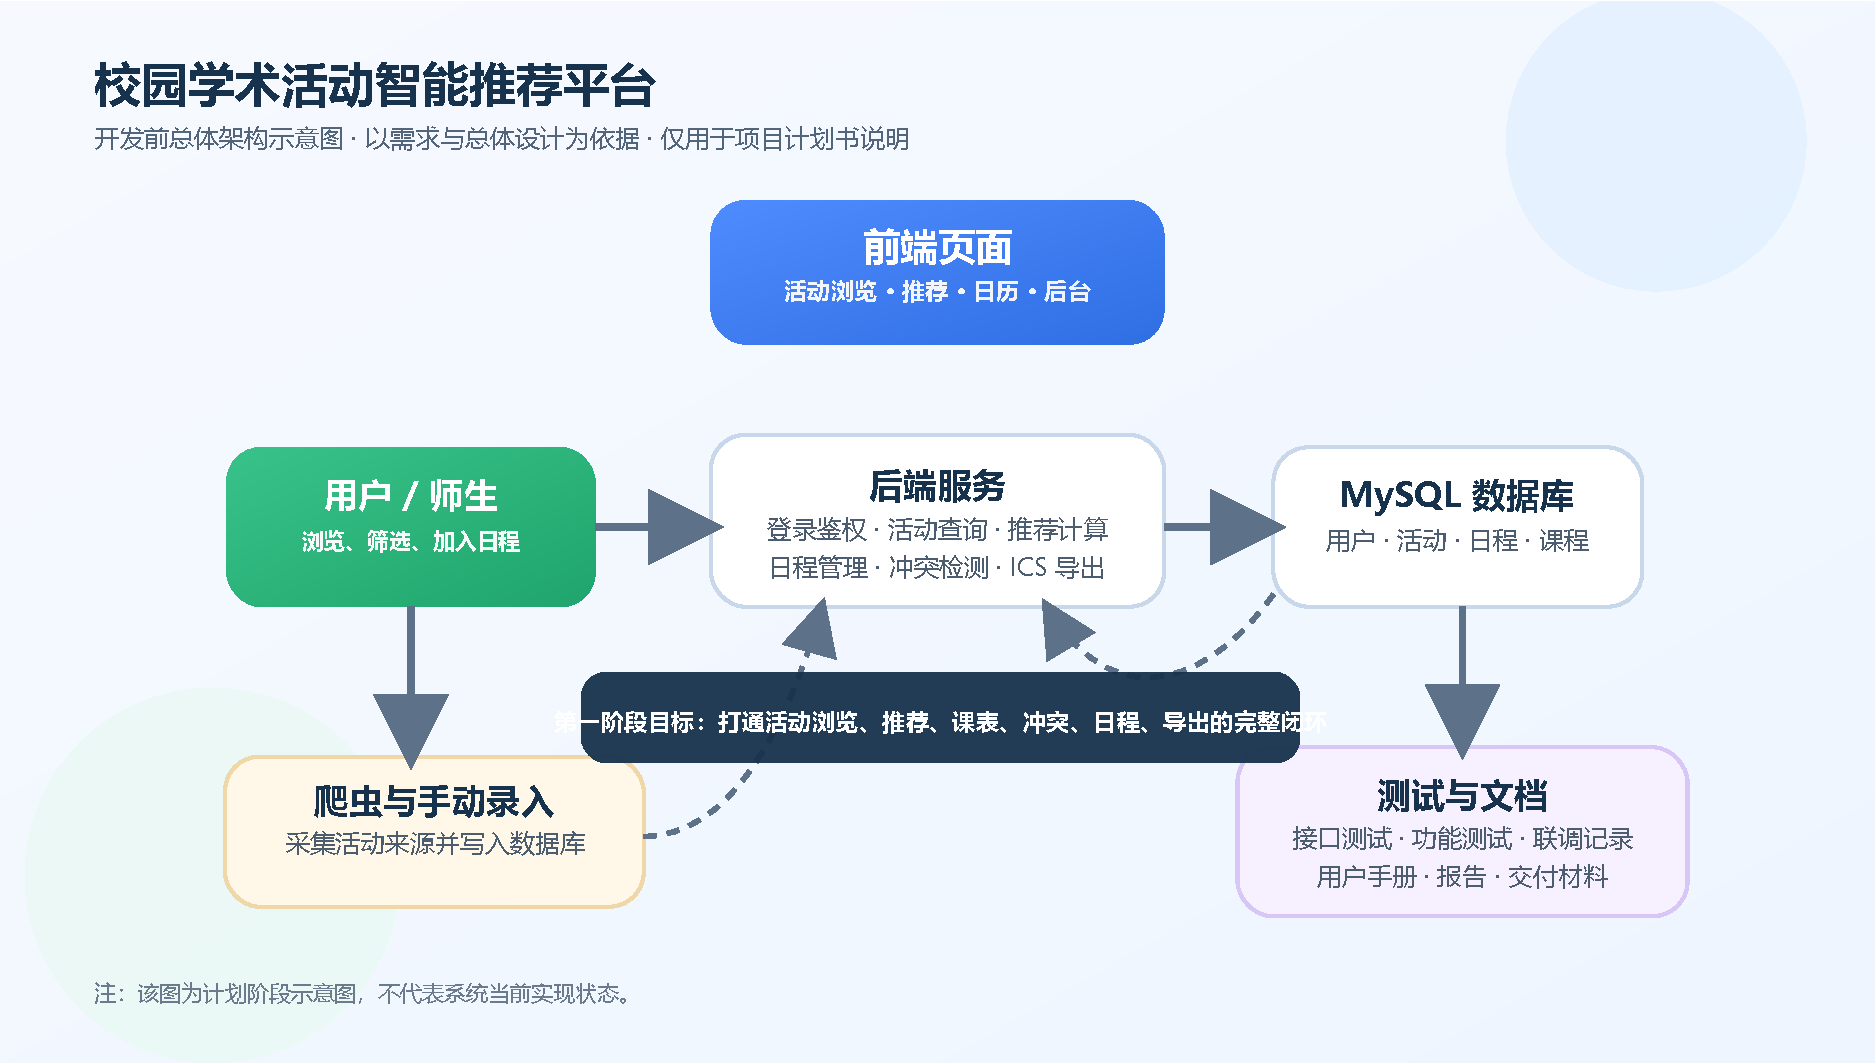
\includegraphics[width=0.92\textwidth]{figures/01-overview.pdf}
\caption{开发目标总体架构示意图}
\end{figure}

\section{前端开发方案}
前端以 Vue 3 + Vite + Element Plus 为基础，围绕“首页推荐、活动列表、活动详情、课表导入、个人日历、后台管理”六个核心页面展开开发。页面开发优先复用既定路由结构，先完成静态交互，再逐步替换为真实接口。

\section{后端开发方案}
后端采用 FastAPI 分层架构，路由层只负责参数接收与响应返回，业务逻辑集中在 \texttt{services/}，数据访问由 \texttt{models/} 与数据库会话层完成。第一阶段优先实现登录注册、用户信息、活动列表、活动详情、推荐、日程、课表导入、后台管理和爬虫记录接口。

\begin{longtable}{|p{0.22\textwidth}|p{0.56\textwidth}|}
\hline
\textbf{模块} & \textbf{主要职责} \\
\hline
\texttt{auth} & 登录、注册、Token 鉴权 \\
\hline
\texttt{users} & 用户信息、兴趣标签、个人中心 \\
\hline
\texttt{activities} & 活动列表、详情、搜索、筛选、排序 \\
\hline
\texttt{recommendations} & 规则推荐、推荐理由 \\
\hline
\texttt{schedules} & 日程查询、加入日程、冲突检测 \\
\hline
\texttt{courses} & 课表导入、课程保存、识别结果接收 \\
\hline
\texttt{admin} & 后台活动管理、爬虫记录、人工修正 \\
\hline
\texttt{crawler} & 爬虫任务触发、运行记录 \\
\hline
\end{longtable}

\section{数据库与爬虫开发方案}
数据库以 \texttt{database/schema.sql} 为权威来源，核心表包括 \texttt{user}、\texttt{activity}、\texttt{activity\_tag}、\texttt{user\_interest}、\texttt{course\_schedule}、\texttt{schedule\_event}、\texttt{registration}、\texttt{crawl\_record}、\texttt{admin\_log}。表结构设计重点保证活动、标签、课程和日程之间的关联关系清晰，便于后续实现推荐与冲突检测。

爬虫部分先完成一个学院或一个数据源的采集闭环，重点实现字段抽取、时间清洗、重复数据去重、入库和运行日志记录。第一阶段以“能稳定产出样例活动数据”为目标，不追求全站覆盖。

\section{测试与文档开发方案}
测试采用“接口测试 + 手工功能测试 + 前后端联调测试 + 演示验收测试”的四层策略。测试负责人统一维护测试用例、Bug 记录和回归结果，确保每次接口变更都能同步到文档和测试清单中。

\begin{figure}[H]
\centering
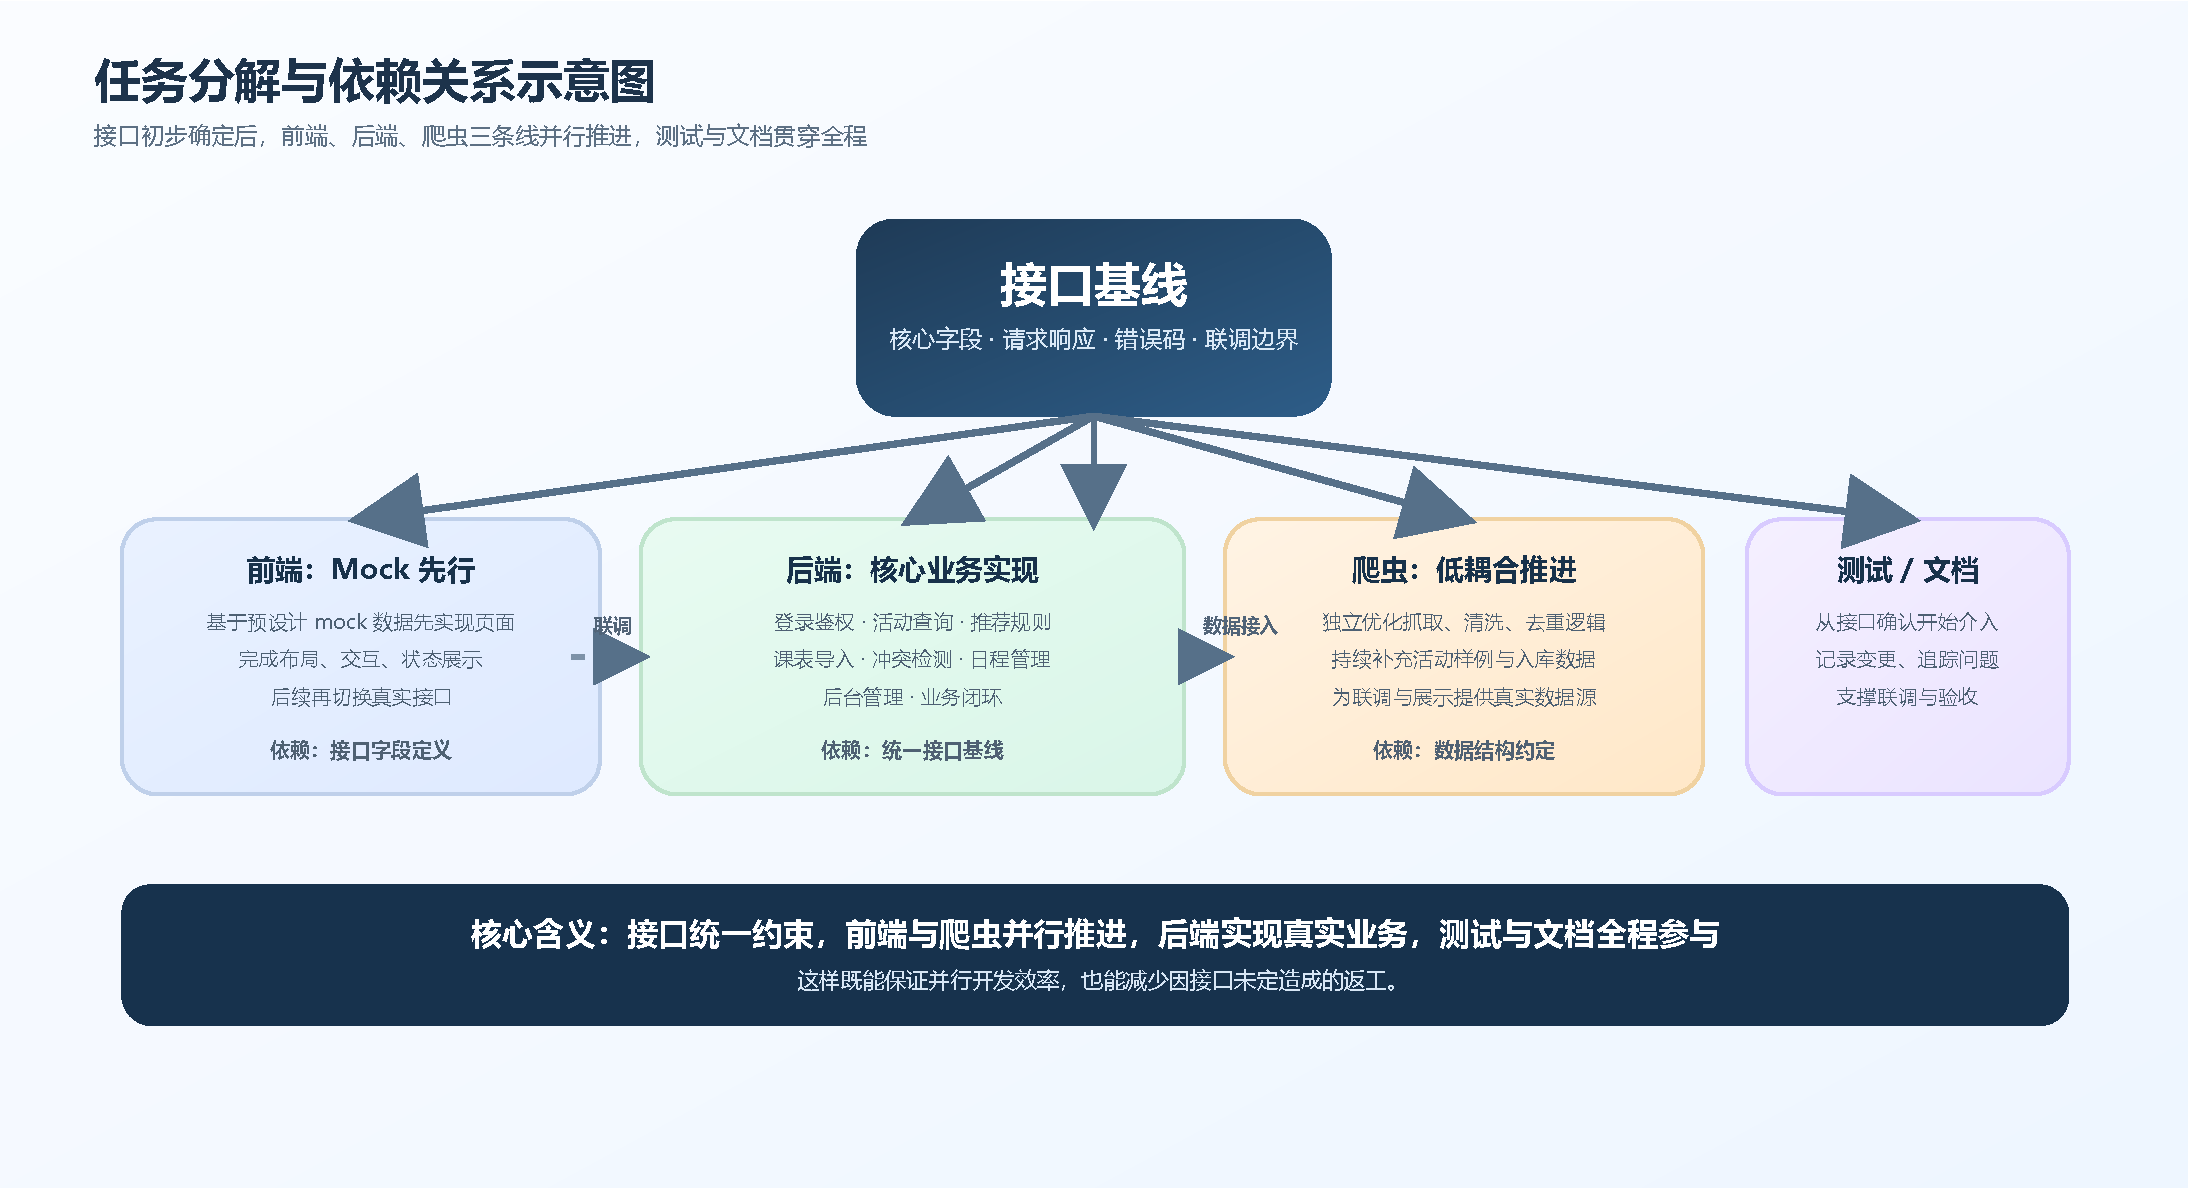
\includegraphics[width=0.92\textwidth]{figures/02-task-dependency-v2.pdf}
\caption{任务分解与依赖关系示意图}
\end{figure}

\chapter{成员分工}

\section{团队角色划分}
我们小组一共6名同学，采用的分工是：1名前端、1名爬虫与数据库、3名后端、1名测试与文书。

\section{成员具体任务}
\begin{longtable}{|p{0.10\textwidth}|p{0.18\textwidth}|p{0.28\textwidth}|p{0.34\textwidth}|}
\hline
\textbf{成员} & \textbf{角色} & \textbf{主要负责内容} & \textbf{交付细则} \\
\hline
朱致远 & 前端负责人 & 页面与交互开发 & 活动列表、活动详情、日历、课表导入、后台页面联调 \\
\hline
宫上珺 & 爬虫与数据库负责人 & 数据来源与数据库设计 & 表结构、种子数据、活动样例数据、计院爬虫与入库 \\
\hline
孟祥烨 & 后端负责人 1 & 后端基础与通用接口 & 数据库连接、ORM 基础、登录注册、用户信息、活动基础接口 \\
\hline
李妍雅 & 后端负责人 2 & 日历与课表业务 & 课表导入、截图识别接口预留、冲突检测、日程、ICS 导出 \\
\hline
庞星磊 & 后端负责人 3 & 推荐与筛选排序 & 活动搜索、标签/类别/校区筛选、排序、推荐规则、后台辅助统计 \\
\hline
黄晗 & 测试与文书负责人 & 测试管理与项目文档 & 测试用例、接口测试、Bug 记录、进度记录、用户手册和报告材料 \\
\hline
\end{longtable}

\chapter{任务分解}

\section{前端任务分解}
前端任务我们大致拟定按照 \textbf{页面骨架 -> 接口接入 -> 交互完善 -> 演示优化} 的思路推进，预期的任务分解和产出如下表：

\begin{longtable}{|p{0.30\textwidth}|p{0.54\textwidth}|}
\hline
\textbf{任务} & \textbf{产出} \\
\hline
登录/注册页面 & 表单校验、登录态保存、路由跳转 \\
\hline
首页推荐页 & 推荐活动卡片、热门活动入口、快捷导航 \\
\hline
活动列表页 & 搜索框、筛选器、分页、排序、空状态 \\
\hline
活动详情页 & 活动信息展示、标签、加入日程入口 \\
\hline
日历页 & 月/周视图、颜色标识、冲突提示 \\
\hline
课表导入页 & 文件上传、识别结果展示、确认入库 \\
\hline
后台管理页 & 活动新增、编辑、下架、爬虫记录查看 \\
\hline
\end{longtable}

\section{后端任务分解}
后端任务按数据层、业务层、接口层依次展开，先实现数据库查询和基础鉴权，再实现业务逻辑和管理接口。

\begin{longtable}{|p{0.30\textwidth}|p{0.54\textwidth}|}
\hline
\textbf{任务} & \textbf{产出} \\
\hline
数据库连接与 ORM & 可复用的 DB 会话、模型和查询封装 \\
\hline
登录注册与鉴权 & \texttt{/auth/login}、Token、\texttt{/users/me} \\
\hline
活动基础接口 & \texttt{/activities}、\texttt{/activities/\{id\}} \\
\hline
推荐规则接口 & 推荐列表、推荐理由、排序规则 \\
\hline
日程与冲突检测 & 冲突判断、日程写入、日历查询 \\
\hline
课表导入接口 & 课程保存、导入结果、OCR 预留 \\
\hline
后台与爬虫接口 & 活动管理、爬虫运行、爬虫记录 \\
\hline
\end{longtable}

\section{爬虫与数据库任务分解}
爬虫与数据库任务的核心目标是建立稳定的数据底座，确保前后端联调时有可用样例数据。

\begin{longtable}{|p{0.30\textwidth}|p{0.54\textwidth}|}
\hline
\textbf{任务} & \textbf{产出} \\
\hline
表结构复核 & 校验字段命名、外键、索引和默认值 \\
\hline
种子数据准备 & 测试账号、测试活动、测试课程样例 \\
\hline
爬虫字段抽取 & 标题、时间、地点、学院、标签、来源链接 \\
\hline
数据清洗去重 & 去除重复活动、统一时间格式、清洗空字段 \\
\hline
入库与日志 & 活动入库、抓取记录、失败信息记录 \\
\hline
\end{longtable}

\section{测试与文档任务分解}
\begin{longtable}{|p{0.30\textwidth}|p{0.54\textwidth}|}
\hline
\textbf{任务} & \textbf{产出} \\
\hline
测试用例设计 & 按模块拆分的测试用例表 \\
\hline
接口测试 & 健康检查、登录、活动列表、日程、管理接口 \\
\hline
联调测试 & 前后端字段对齐、错误处理、边界条件修复 \\
\hline
文档维护 & 进度记录、测试报告、用户手册、接口文档同步 \\
\hline
\end{longtable}

\section{任务依赖关系}
简单来说，在接口初步确定好之后，前端负责的同学可以先利用预先设计的一版 mock 数据进行前端页面实现，而爬虫负责的同学的同样可以相对低耦合的去实现和优化爬取数据的处理逻辑。后端的同学则着手实现核心业务。测试和文档维护则贯穿开发始终。

\begin{figure}[H]
\centering
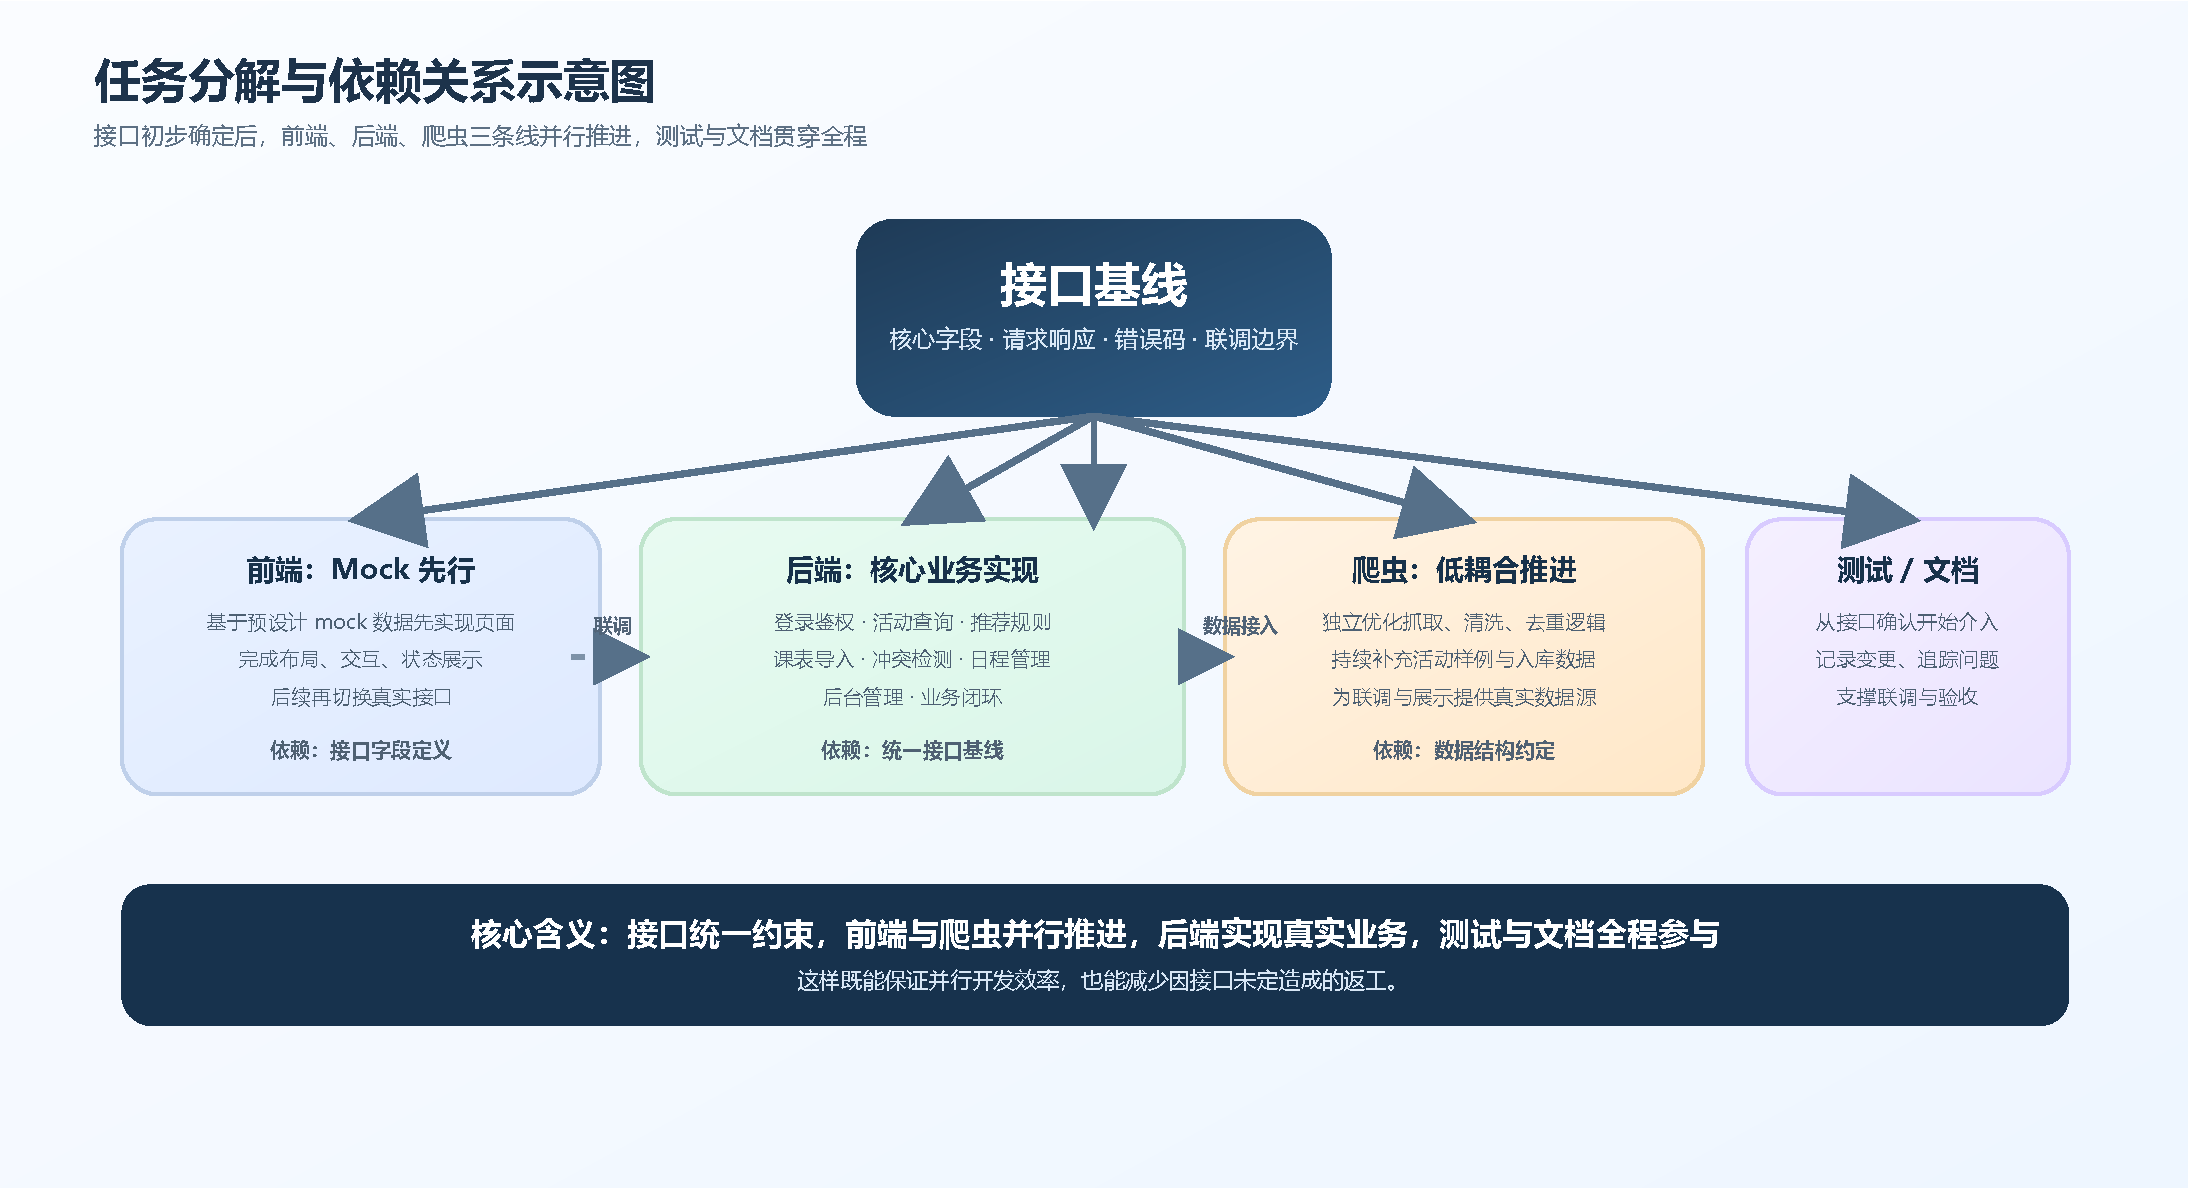
\includegraphics[width=0.95\textwidth]{figures/02-task-dependency-v2.pdf}
\caption{任务分解与依赖关系示意图}
\end{figure}

\chapter{进度安排}

\section{总体排期}
\begin{longtable}{|p{0.16\textwidth}|p{0.18\textwidth}|p{0.24\textwidth}|p{0.30\textwidth}|}
\hline
\textbf{阶段} & \textbf{拟定周期} & \textbf{核心目标} & \textbf{主要产出} \\
\hline
第一阶段 & 4--5 天 & 数据与基础接口优先 & 稳定表结构、登录、活动列表、详情接口 \\
\hline
第二阶段 & 3--5 天 & 主流程联调 & 搜索筛选、推荐、课表导入、冲突检测、日程写入 \\
\hline
第三阶段 & 4--5 天 & 演示闭环补齐 & ICS 导出、后台管理、页面细节、异常处理 \\
\hline
第四阶段 & 2--3 天 & 测试与交付准备 & 测试报告、用户手册、答辩材料、Bug 收敛 \\
\hline
\end{longtable}

\begin{figure}[H]
\centering
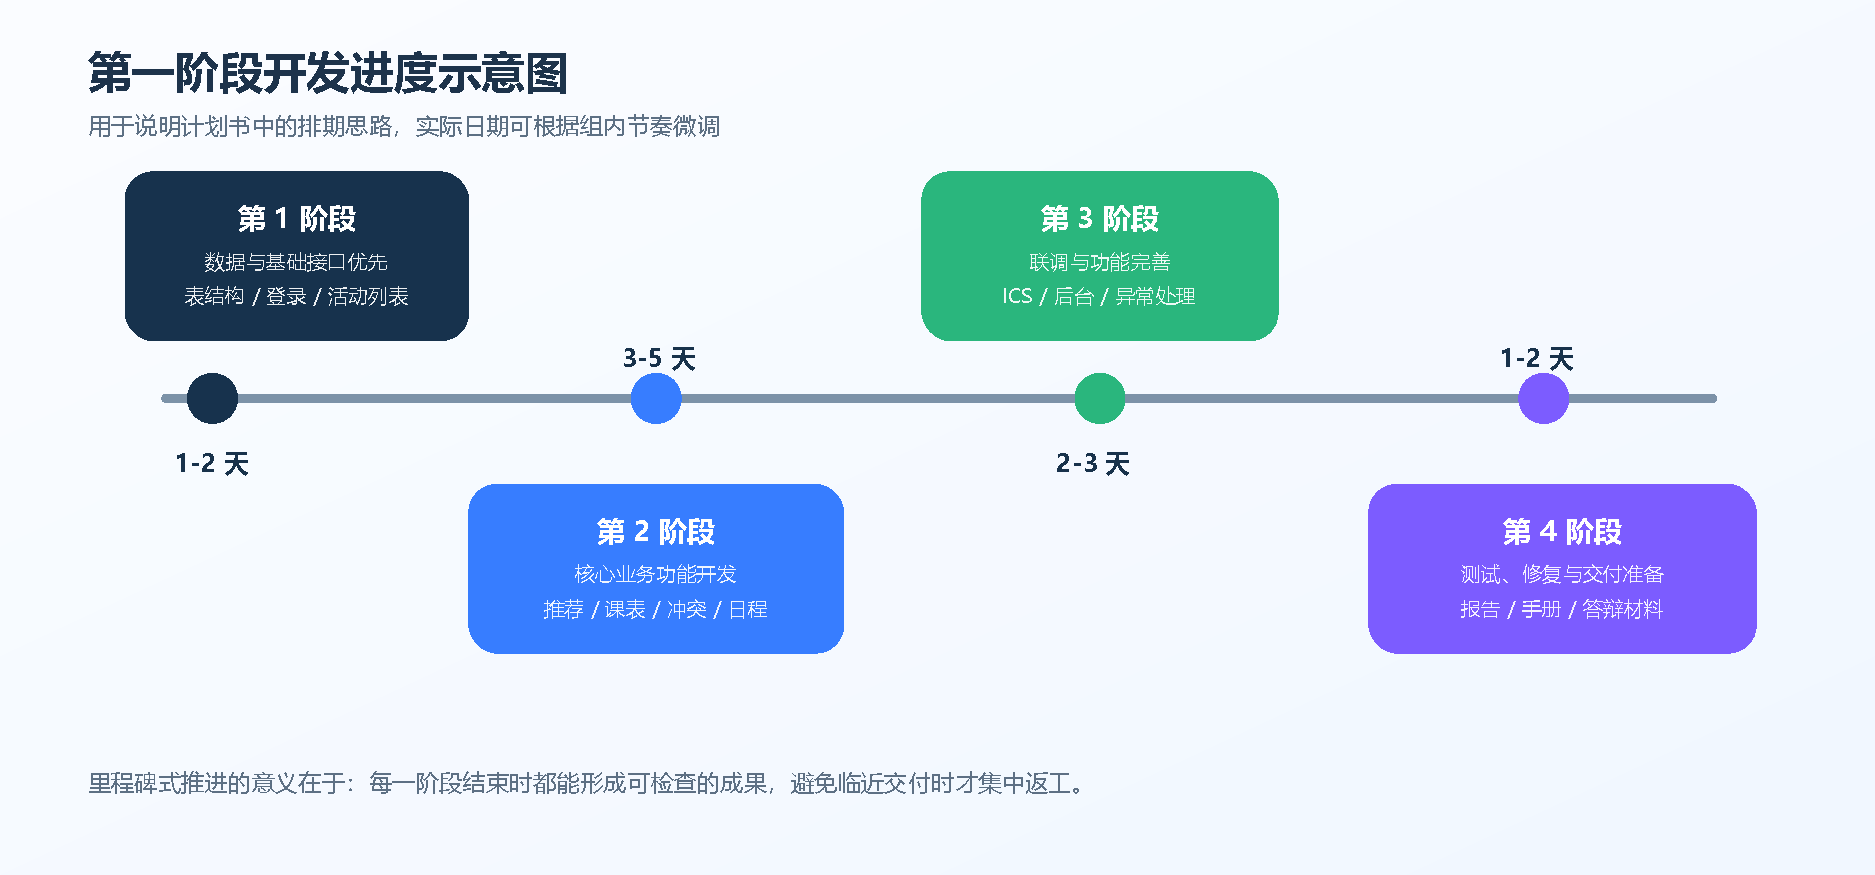
\includegraphics[width=0.95\textwidth]{figures/04-timeline.pdf}
\caption{第一阶段开发进度示意图}
\end{figure}

\section{第一阶段：项目初始化与基础链路}
\begin{longtable}{|p{0.16\textwidth}|p{0.74\textwidth}|}
\hline
\textbf{成员} & \textbf{任务} \\
\hline
gsj & 稳定数据库表结构，补充种子数据，整理字段说明 \\
\hline
mxy & 完成数据库连接、ORM 基础、用户登录、用户信息、活动列表和详情接口 \\
\hline
hh & 建立测试用例骨架，记录字段和接口变更 \\
\hline
zzy & 基于页面骨架完成活动列表、详情、登录页的联调准备 \\
\hline
pxl & 确认筛选和推荐所需字段，给出推荐分第一版规则 \\
\hline
lyy & 确认日程和课程表字段，设计冲突检测输入输出 \\
\hline
\end{longtable}

阶段完成标志：前端能调用真实活动列表接口，后端能从 MySQL 返回活动数据，测试同学能跑通健康检查、登录和活动列表。

\section{第二阶段：核心业务功能开发}
\begin{longtable}{|p{0.16\textwidth}|p{0.74\textwidth}|}
\hline
\textbf{成员} & \textbf{任务} \\
\hline
zzy & 对接登录、活动列表、活动详情、推荐活动、日历事件接口 \\
\hline
gsj & 完成第一版爬虫数据解析，准备活动样例数据入库 \\
\hline
mxy & 完成注册、JWT 鉴权依赖、后台活动新增/编辑/下架基础接口 \\
\hline
lyy & 完成课程录入、CSV/Excel 导入、日程查询、冲突检测、加入日程 \\
\hline
pxl & 完成关键词搜索、类别/标签/校区筛选、热度/时间/推荐分排序 \\
\hline
hh & 开始执行接口测试和前后端联调测试，记录 Bug 和复现步骤 \\
\hline
\end{longtable}

阶段完成标志：用户可以登录，可以浏览和筛选活动，可以查看活动详情，可以导入或录入课程，可以检测活动与课程冲突，可以把活动加入日程并在日历中看到。

\section{第三阶段：联调与功能完善}
\begin{longtable}{|p{0.16\textwidth}|p{0.74\textwidth}|}
\hline
\textbf{成员} & \textbf{任务} \\
\hline
zzy & 完成页面交互细节、状态标签、错误提示和演示截图 \\
\hline
gsj & 修正爬虫清洗和去重，保证演示数据质量 \\
\hline
mxy & 完善错误响应、权限判断、管理员接口稳定性 \\
\hline
lyy & 完成 ICS 导出，OCR 接口可根据时间做预留或简化演示 \\
\hline
pxl & 调整推荐理由和推荐排序，补充后台统计接口 \\
\hline
hh & 完成第一轮系统测试、测试报告初稿、用户手册初稿 \\
\hline
\end{longtable}

阶段完成标志：答辩演示主流程可以连续跑通，测试报告有执行记录，用户手册能指导普通用户和管理员完成核心操作。

\section{第四阶段：测试、修复与交付准备}
\begin{longtable}{|p{0.16\textwidth}|p{0.74\textwidth}|}
\hline
\textbf{成员} & \textbf{任务} \\
\hline
全体 & 修复高优先级 Bug，统一演示环境，确认代码合并状态 \\
\hline
zzy & 准备前端展示截图和演示流程说明 \\
\hline
gsj & 准备数据库 ER 图、活动数据来源说明、爬虫运行截图 \\
\hline
mxy、lyy、pxl & 准备后端接口、核心逻辑和 Swagger 截图 \\
\hline
hh & 汇总测试报告、用户手册、进度文档和答辩材料 \\
\hline
\end{longtable}

\chapter{阶段性里程碑}
这部分其实就对应了上一节的分阶段进度安排，这里不过多赘述，仅仅简要阐释完成标准。
\begin{longtable}{|p{0.16\textwidth}|p{0.28\textwidth}|p{0.48\textwidth}|}
\hline
\textbf{里程碑} & \textbf{内容} & \textbf{完成标准} \\
\hline
一 & 项目骨架与数据库完成 & 数据库建表、测试数据、后端基础配置和前端路由骨架全部可用 \\
\hline
二 & 活动浏览主链路完成 & 活动列表、详情页、分页、搜索和基础推荐可联调 \\
\hline
三 & 日历与冲突检测完成 & 课表导入、日程展示、冲突提示和加入日程可以闭环 \\
\hline
四 & 完整演示流程完成 & 从登录到导出 ICS 的主流程可连续演示，无阻断问题 \\
\hline
五 & 最终交付版本完成 & 代码、数据库、文档、测试报告和答辩材料统一归档，可提交 \\
\hline
\end{longtable}

\chapter{协作方式}

\section{Git 协作规范}
项目采用 \texttt{main} 稳定主分支，开发时按模块建立功能分支，暂定规范如下：

\begin{verbatim}
main                        # 稳定主分支
frontend/xxx                # 前端功能
backend/xxx                 # 后端功能
crawler/xxx                 # 爬虫功能
database/xxx                # 数据库相关
docs/xxx                    # 文档相关
test/xxx                    # 测试相关
fix/xxx                     # Bug 修复
\end{verbatim}

\begin{figure}[H]
\centering
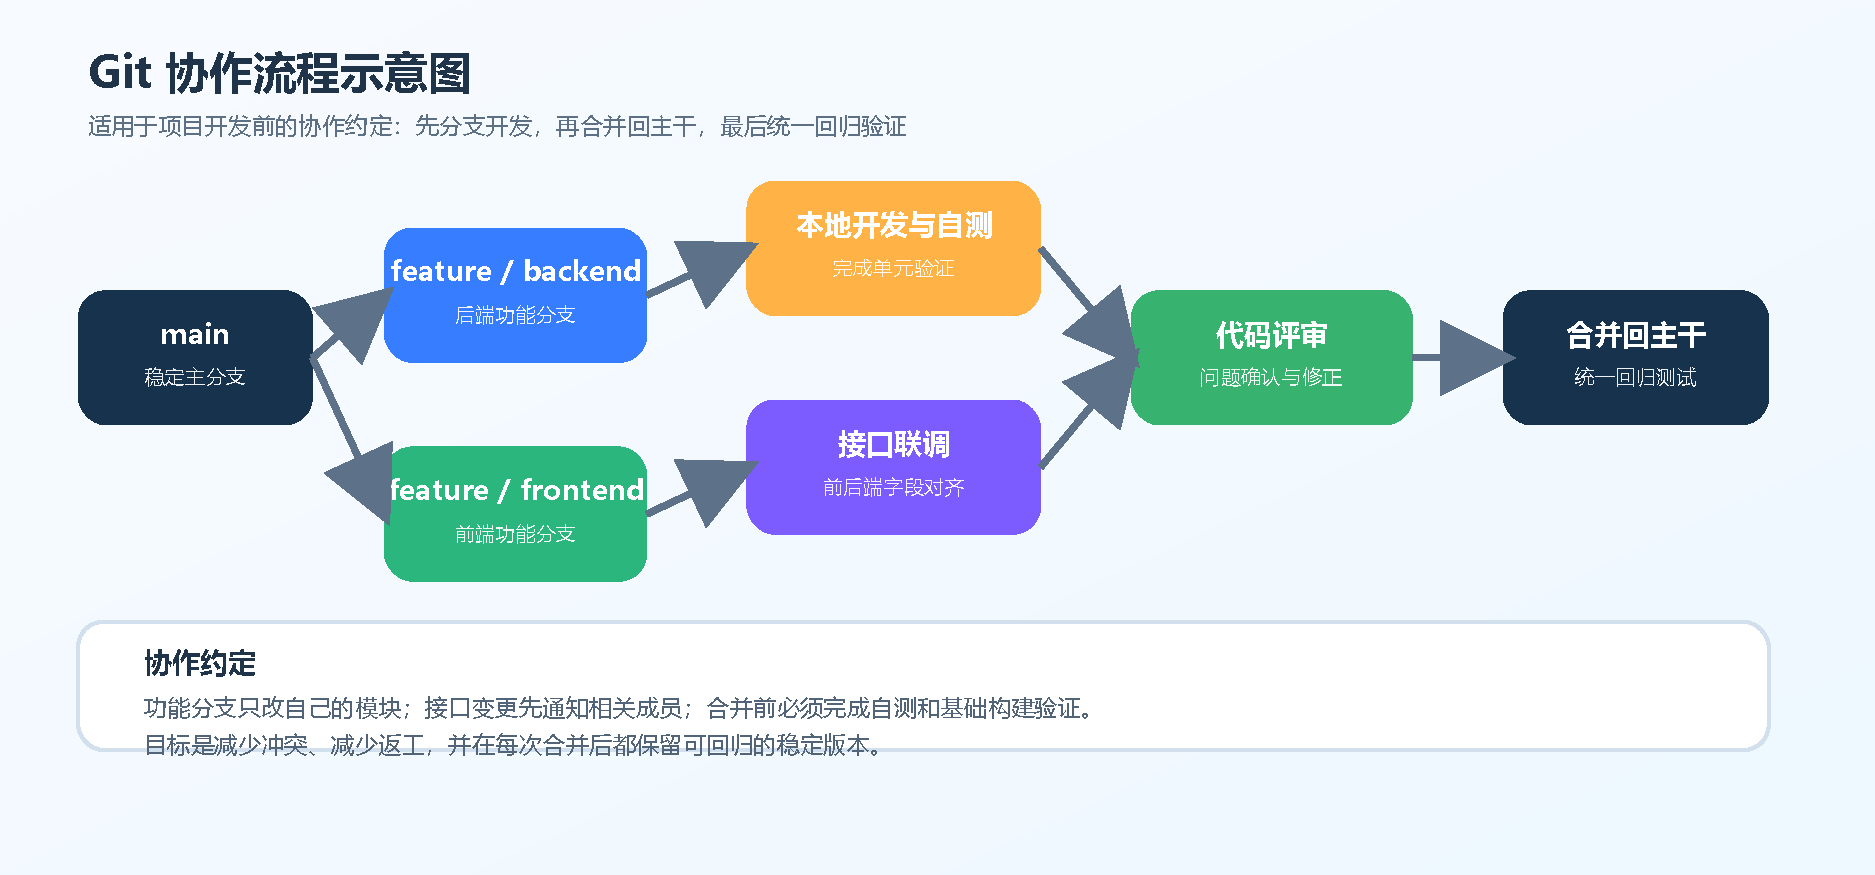
\includegraphics[width=0.88\textwidth]{figures/03-git-workflow.pdf}
\caption{Git 协作流程示意图}
\end{figure}

\noindent 同时我们规定的 commit 提交的信息规范，方便组员之间对齐进度，知道对方现在做到哪里了：

\begin{longtable}{|p{0.12\textwidth}|p{0.20\textwidth}|p{0.48\textwidth}|}
\hline
\textbf{类型} & \textbf{含义} & \textbf{示例} \\
\hline
feat & 新增功能 & \texttt{feat: add activity list page} \\
\hline
fix & 修复 Bug & \texttt{fix: fix schedule conflict check} \\
\hline
doc & 文档修改 & \texttt{docs: update environment setup guide} \\
\hline
style & 样式调整，不影响逻辑 & \texttt{style: polish login page layout} \\
\hline
refactor & 重构代码，不新增功能 & \texttt{refactor: split activity service} \\
\hline
test & 测试相关 & \texttt{test: add auth api tests} \\
\hline
chore & 配置、依赖、脚手架等杂项 & \texttt{chore: update gitignore} \\
\hline
build & 构建或打包配置 & \texttt{build: add frontend dockerfile} \\
\hline
ci & CI/CD 配置 & \texttt{ci: add github actions workflow} \\
\hline
\end{longtable}

\section{分支管理规范}
\begin{enumerate}[leftmargin=2.5em]
\item 每个功能尽量只改自己的模块，避免无关文件互相覆盖。
\item 合并前必须完成本地测试或基础构建验证。
\item 与接口相关的变更必须同步通知前端、测试和文档负责人。
\end{enumerate}

\section{文档同步规范}
开发过程中的关键文档包括 \texttt{docs/api-contract.md}、\texttt{docs/test-plan.md}、\texttt{docs/test-cases.md}、\texttt{docs/user-manual.md} 和 \texttt{progress/} 下的进度记录。所有影响用户操作或接口结构的改动，都应在对应文档中留下记录。

\section{组员沟通联络}
我们按照任务进度定期线上会议对进度，借助腾讯会议并且回放留档。在日常开发过程中我们则通过微信群直接联络，及时 update 个人任务。GitHub 上的项目 \texttt{docs/} 目录下面用于记录项目相关的各种文档及规范，直接替代共享文档。

\chapter{测试与验收计划}

\section{功能测试计划}
\begin{longtable}{|p{0.20\textwidth}|p{0.66\textwidth}|}
\hline
\textbf{测试模块} & \textbf{重点检查内容} \\
\hline
登录注册 & 正常登录、错误密码、Token 失效 \\
\hline
活动列表 & 分页、筛选、排序、空状态 \\
\hline
活动详情 & 数据完整性、标签展示、加入入口 \\
\hline
课表导入 & 文件格式、导入结果、错误提示 \\
\hline
冲突检测 & 与课程冲突、与已有日程冲突 \\
\hline
日程与日历 & 事件展示、颜色标识、状态标签 \\
\hline
后台管理 & 新增、编辑、下架、记录查看 \\
\hline
\end{longtable}

\section{接口测试计划}
接口测试优先覆盖健康检查、登录、活动列表、活动详情、推荐、日程、课表导入、后台活动管理和爬虫记录接口。接口测试结果应保留请求参数、返回内容和执行时间，便于回归对比。

\section{联调测试计划}
联调阶段重点检查前后端字段是否一致、空数据是否能正确展示、异常返回是否能被前端友好处理、冲突弹窗是否能正确触发。

\section{验收演示流程}
目前拟定的演示流程为：
\begin{enumerate}[leftmargin=2.5em]
\item 登录系统。
\item 进入首页查看推荐。
\item 打开活动列表并进行筛选。
\item 查看活动详情。
\item 导入课表并生成日程。
\item 点击加入活动，触发冲突检测。
\item 在日历中查看活动与课程。
\item 导出 ICS 文件。
\item 进入后台维护活动并查看爬虫记录。
\end{enumerate}

\chapter{风险与应对措施}
\begin{longtable}{|p{0.18\textwidth}|p{0.28\textwidth}|p{0.38\textwidth}|}
\hline
\textbf{风险类型} & \textbf{具体表现} & \textbf{应对措施} \\
\hline
技术风险 & 后端接口较多、实现进度慢 & 优先实现主流程接口，先保证可联调 \\
\hline
进度风险 & 某一模块拖慢整体集成 & 按里程碑推进，设置交接节点 \\
\hline
数据风险 & 样例活动过少或字段不统一 & 提前冻结字段，补充种子数据 \\
\hline
联调风险 & 前后端字段不一致 & 接口先行，变更同步到文档与测试 \\
\hline
展示风险 & 演示时数据不足或流程中断 & 提前准备演示数据和备用流程 \\
\hline
\end{longtable}

\chapter{交付计划}

\section{代码交付}
交付内容包括前端源码、后端源码、爬虫代码、数据库脚本和测试代码。代码应保证可以通过项目现有启动方式运行。

\section{数据库交付}
交付内容包括 \texttt{database/schema.sql}、\texttt{database/seed.sql} 和必要的字段说明，确保他人可重新初始化数据库并复现实验环境。

\section{文档交付}
交付文档包括开发计划书、总体设计报告、接口文档、测试计划、测试用例、测试报告、用户手册和进度记录。

\section{演示交付}
演示交付要求准备稳定的演示数据、可访问的接口、可展示的截图和可重复的主流程脚本，保证答辩现场不依赖临时修改。

\end{document}
